% !TEX encoding = UTF-8 Unicode
% !TEX root = DesignDocument.tex

\documentclass{book}

% !TEX root = DesignDocument.tex



\usepackage[width=6.5in, height=9.2in, top=1.0in, papersize={8.5in,11in}]{geometry}
\usepackage[pdftex]{graphicx}
\usepackage{amsmath}
\usepackage{amsthm}
\usepackage{amssymb}
%\usepackage{txfonts}
\usepackage{textcomp}
\usepackage{amsthm}
\usepackage{algpseudocode}
\usepackage{fancyhdr}
\pagestyle{fancy}
\usepackage{hyperref}
\usepackage{verbatim}


\usepackage{array}
\usepackage{color}
\usepackage{listings}
\usepackage{calc}
\usepackage[utf8]{inputenc}
\usepackage{makeidx}
\usepackage{multicol}
\usepackage{multirow}
\usepackage[table]{xcolor}
\usepackage{tabularx}
\usepackage{framed}
\usepackage{xspace}
\usepackage{etex}
\usepackage{todonotes}


%% Computer Modern Bright Font
%\usepackage{cmbright}
%\usepackage[T1]{fontenc}

%% Sans Serif Modern Font - similar to  Helvetica
\usepackage{lmodern}
\renewcommand*\familydefault{\sfdefault} %% Only if the base font of the document is to be sans serif
\usepackage[T1]{fontenc}


\definecolor{SDColor1}{rgb}{0,0,0}
\definecolor{SDColor2}{rgb}{0,0,0}
\definecolor{SDColor3}{rgb}{0,0,0}
\definecolor{SDColor4}{rgb}{0,0,0}
\definecolor{SDColor5}{rgb}{0,0,0}

%%%  --- Here are some other colors.  Keep it conservative --- %%%

%% Blue font color scheme
%\definecolor{SDColor1}{rgb}{.204,.353,.541}
%\definecolor{SDColor2}{rgb}{.31,.506,.741}
%\definecolor{SDColor3}{rgb}{0.18,0.35,0.59}
%\definecolor{SDColor4}{rgb}{0.44,0.59,0.82}
%\definecolor{SDColor5}{rgb}{0.35,0.35,0.35}
%

% Brown color scheme
% \definecolor{SDColor1}{rgb}{.55,.2,.2}
%\definecolor{SDColor2}{rgb}{.4,.1,.1}
%\definecolor{SDColor3}{rgb}{.5, .15,.15}
%\definecolor{SDColor4}{rgb}{.63,.32,.18}
%\definecolor{SDColor5}{rgb}{.45,.15,.15}
%


%% Custom colors for code listing environment
\definecolor{OliveGreen}{cmyk}{0.64,0,0.95,0.40}
\definecolor{DarkBlue}{cmyk}{0.76,0.76,0,0.20}
\definecolor{DarkRed}{cmyk}{0,1,1,0.45}
\lstset{language=c,frame=ltrb,framesep=5pt,basicstyle=\normalsize,
 keywordstyle=\ttfamily\color{DarkRed},
identifierstyle=\ttfamily\color{DarkBlue}\bfseries,
commentstyle=\color{OliveGreen},
stringstyle=\ttfamily,
showstringspaces=false,tabsize = 3}


\setlength{\oddsidemargin}{0mm} 
\setlength{\evensidemargin}{0mm} 

%% Uncomment if you want "Draft" placed on each page.
%\usepackage{draftwatermark}
%\SetWatermarkLightness{0.975}
%\SetWatermarkScale{1}
%\SetWatermarkText{Draft}

\pagestyle{fancy}
\renewcommand{\chaptermark}[1]{\markboth{#1}{}}
\renewcommand{\sectionmark}[1]{\markright{\thesection\ #1}}
\fancyhf{}
\fancyhead[LE,RO]{\bfseries\thepage}
\fancyhead[LO]{\bfseries\rightmark}
\fancyhead[RE]{\bfseries\leftmark}
%\fancyfoot[LE,RO]{Confidential and Proprietary}
%\renewcommand{\headrulewidth}{0.5pt}
%\renewcommand{\footrulewidth}{0pt}
%\addtolength{\headheight}{0.5pt}
%\setlength{\footskip}{0mm}
%\renewcommand{\footruleskip}{0pt}



\usepackage{titlesec}
\titleformat{\chapter}[display]
{\normalfont\bfseries\color{SDColor3}}    %\normalfont\bfseries\filcenter}
{\LARGE\thechapter}
{1ex}
{\titlerule[2pt]
\vspace{2ex}%
\LARGE}
[\vspace{1ex}%
{\titlerule[2pt]}]

%
%\usepackage{titlesec}
%\titleformat{\chapter}{\normalfont\bfseries\LARGE}
%{\thechapter.}{5pt}{}[{\titlerule[3pt]}]
%
%\titleformat{\section}{\normalfont\bfseries\Large}
%{\thesection.}{5pt}{}[{\titlerule[2pt]}]
%
%\titleformat{\subsection}{\normalfont\bfseries\large}
%{\thesubsection.}{5pt}{}[{\titlerule[1pt]}]
%


%\titleformat*{\section}{\Large\bfseries\sffamily\color{SDColor1}}
%\titleformat*{\subsection}{\large\bfseries\sffamily\color{MSLightBlue}}
%\titleformat*{\section}{\Large\bfseries\color{SDColor3}}
%\titleformat*{\subsection}{\large\bfseries\color{SDColor4}}

%\titleformat*{\section}{\Large\bfseries}
%\titleformat*{\subsection}{\large\bfseries}
%\titleformat*{\subsubsection}{\large\bfseries}

\titleformat*{\section}{\Large\bfseries\color{SDColor1}}  
\titleformat*{\subsection}{\large\bfseries\color{SDColor2}}
\titleformat*{\subsubsection}{\large\bfseries\color{SDColor5}}
\setcounter{secnumdepth}{3}
\renewcommand{\thesubsubsection}{\thesubsection.\alph{subsubsection}}

% Save the original chapter command as stdchapter
\let\stdchapter\chapter

%redefine the backmatter command
\let\stdbackmatter\backmatter
\makeatletter% We need the '@' letter to call if@openright
\renewcommand{\backmatter}{
\stdbackmatter
% need to set the page counter back to 1
\setcounter{page}{1}
%% Redefine the \chapter command for our Back Matter
\renewcommand{\chapter}[1]{
  \if@openright\cleardoublepage\else\clearpage\fi% chapters begin on right page
  \stdchapter{##1}% output standard chapter heading
  \setcounter{section}{0}% restart the section numbering
  \renewcommand{\thepage}{BM-\arabic{page}}% Redefine page numbering format
  \renewcommand{\thesection}{\arabic{section}}% Redefine section number format
}}
\makeatother% Restore the normal behavior of '@'

%redefine the appendix command
\let\stdappendix\appendix
\makeatletter% We need the '@' letter to call if@openright
\renewcommand{\appendix}{
\stdappendix
%% \titleformat{\chapter}[display]
%% {\normalfont\bfseries\color{SDColor3}}    %\normalfont\bfseries\filcenter}
%% {\LARGE Appendix \thechapter}
%% {1ex}
%% {\titlerule[2pt]
%% \vspace{2ex}%
%% \LARGE}
%% [\vspace{1ex}%
%% {\titlerule[2pt]}]
  %%% Since counters are different in the appendix section
  %%% we redefine \chapter to explicitly reset the page number
  %%%  (comment out to see effect)
  \renewcommand{\chapter}[1]{
    \stdchapter{##1}\setcounter{page}{1}
    %%% We also redefine page numbering
    \renewcommand{\thepage}{\Alph{chapter}-\arabic{page}}
  }
}
\makeatother% Restore the normal behavior of '@'


\makeatletter% We need the '@' letter to call if@openright
\newcommand{\agreement}{
  \renewcommand{\chapter}[1]{
    \if@openright\cleardoublepage\else\clearpage\fi% chapters begin on right page
    \pagestyle{plain}% turn off fancy headers
    \setcounter{section}{0}% Reset the section number
    \setcounter{page}{1}% Reset the page number
    \renewcommand{\thepage}{SA-\arabic{page}}% Set format for page numbering
    \renewcommand{\thesection}{\arabic{section}}% Set format for section numbering
    \refstepcounter{chapter}% Add it to the index/toc for on-line viewing
    \addcontentsline{toc}{chapter}{##1}% Add to the table of contents
  }
}
\makeatother% Restore the normal behavior of '@'



%%  If you do some math typesetting, you may want more environment names.
%% Uncomment to see how this works:
%\newtheorem{summary}{Summary:}
%\newtheorem{example}{Example:}



 % This sets the format.

% Add your title page contents here 
\title{{\color{SDColor3} \rule{\linewidth}{0.5mm}}\\[2mm] {\huge \bfseries \color{SDColor3} CSC412 Cryptography Portfolio }\\[-1mm] {\color{SDColor3}\rule{\linewidth}{0.5mm}} \\  \vfill
{\LARGE \bfseries \color{SDColor4} Project Documentation and Narrative}\\  \vfill }
\author{\color{SDColor3}  Zachary Owen}
\date{\color{SDColor3} \today}


\begin{document}

\frontmatter

\addcontentsline{toc}{chapter}{Title}
\maketitle
\tableofcontents
\addcontentsline{toc}{chapter}{Contents}

\listoffigures
\addcontentsline{toc}{chapter}{List of Figures}
\listoftables
\addcontentsline{toc}{chapter}{List of Tables}

%\listofalgorithms
%\addcontentsline{toc}{chapter}{List of Algorithms}

\mainmatter

% !TEX root = DesignDocument.tex


\chapter{Overview and  Description }

\section{Team Members and Team Name}
RITA Dev Team
\begin{itemize}
\item Logan Lembke: Intern at Black Hills Information Security
\item Zachary Owen: Computer Science Student
\end{itemize}

\section{Client}

\section{Project}

\subsection{Mission Statement}
\subsection{Elevator Pitch}

\subsection{Purpose of the System}
Any exploratory data analysis will be used to guide the actual analytics used within RITA.


% !TEX root = DesignDocument.tex

\chapter{Classic CryptoSystems}

\section{Affine Cipher}

The Affine Cipher is an example of a simple shift cipher and one of the oldest examples of cryptography.
The cipher is performed by transforming each character with the function $f(x) = \alpha x + \beta \pmod{26}$.
Letters are represented as nubers taking each character in the plaintext as a number from 0 to 25, with $a$ being 0, and $z= 25$.

The 'key' to this cipher is choosing $\alpha$ and $\beta$. It is also where a naive implementation of this cipher can fail.
Since the modualar arithmetic system we are working in is not prime the affine cipher is not a feild. 
This means that depending on our choice of $\alpha$ and $\beta$ ( or as it turns out just $\alpha$ ) we could end up with an ambigious cryptosystem.
For example for $\alpha = 13$ the letters n, p, l, t, and r all map to the same letter Making the message very difficult to recover.
So for a funcitional affine system it is necessary that $f(x)$ be a one-to-one function. 
This can be done easily by checking that $gcd(\alpha , 26) = 1$, if this is true then $\frac{1}{\alpha}$ exists and is unique.

\subsection{implementation}
The affine cipher provided is implemented in python for the basic setup and greatest common divisor checking.
The input is then run through a sed transform command that performs the cipher.
Decryption is done much the same way except the transform arguments are reversed.

\section{Vigen\'ere Cipher}

The Vigen\'ere Cipher is a simple cipher from the 16th century. 
The way it functions is also rather simple.
From a given keyword the value of the first letter of the plaintext is added to the value of the first letter of the key. 
The value of the letter being its iteger representaion mod 26.
This continues until the end of the key. At which point you start over with the begining of the key until the end of the plaintext.
The resultant representations of numbers mod 26 are then converted back into letters and sent as the ciphertext.

Decyption is simple if you know the key. 
Simply by undoing the operation of encryption by subtracting the value of each letter of the key mod 26 the plaintext is reaquired.

\subsection{ Implementation}

Included is a C++ implementation of the Vigen\'ere cipher.
The implementation is much the same as it is decribed above.
The Vigen\'ere is built by navigating to \textit{Cryptosuite/vigenere} and running \textbf{make}. This builds \textit{attack}, \textit{decrypt} and \textit{encrypt}.

\section{Frequency Calulator}
The frequency calculator creates an array of 26 ints. It then reads from \textbf{stdin} until \textbf{EOF} is reached and then prints the frequencies.

\section{Affine Cipher Attack}

The affine cipher main problem (besides the existence of only 312 keys) is that it is frequency attacks.
While known plaintext attacks are amazingly effective, with large enough ciphertext it is possible to break most affine ciphers.
The attack provided works by calculating the frequency of each letter in the cipher text and then assuming the letter with the greatest frequency is 'e'.
From there the algebra is simple to find $\alpha$ and $\beta$.


\section{Vigen\'ere Cipher Attacks}

Attacks on Vigen\'ere are more subtle than Affine.
Since each letter is offset by a diffrent ammount basic frequency analysis will ususally yeild garbage and will not give you the key.
instead the attack is performed in two steps

\subsection{Find the key length}
While not basic frequency analysis this method works on the same principle.
The idea is that if the cipher text is placed next to itself plus some offset and then the letters are compared side by side, 
the offset with the most sets of letters in common will be the key length.
This is not freqency analysis but since we know that letters like 'e' and 't' are very common more matches will be found if the letters are mapped to the same place.

This works very well on all but very short ciphertexts.
An interesting result is that for short keys, the side-by-side matching tends to suspect keylengths in multiples of the actual keylength.
This is however unimportant due to the nature of the cipher.

\subsection{ Find the Key}

Now that we know the key length finding the key is no harder than finding the key for the Affine cipher.
In my implementation the ciphertext is partitioned by suspected key length offset and placed into buckets.
Frequency analysis is then performed on each of those buckets and it is assumed that the largest character is 'e'.
The program then simply finds the key character necessary to make that character 'e' and cobbles together a key.

This sort of analysis can be fooled by intentional avoidance of the letter 'e' or by making sure not enough ciphertext encrypted by a single key is sent.
These are odd use cases however and the attacks provided usually work.

\subsection{ Implementation}

Included is a C++ implementation of the Vigen\'ere cipher attack. 
The implementation is much the same as it is decribed above.
The Vigen\'ere attack is built by navigating to \textit{Cryptosuite/vigenere} and running \textbf{make}. This builds \textit{encrypt}, \textit{decrypt} and \textit{attack}.

Running this program is as simple as running \textit{\$ ./attack < <ciphertext> }. The program will then print the guessed size of the key along with the guessed key.

\section{ADFGX cipher}

During the first World War two simmilar ciphers were used called playfair and ADFGX. 
These ciphers worked by placing all possible letters into a grid that could then be used as a one-to-one function.
The indexes of the letter to encrypt were then taken and scrambled in a way that is very difficult to undo without the key.
Like vigen\'ere the key is a word or unique collection of letters.

\subsection{ Description of Algorithm }

\begin{table}[ht]
\centering
\begin{tabular}{ c c c c c }
p&g&c&e&n \\
p&q&o&z&r \\
s&l&a&f&t \\
m&d&v&i&w \\
k&u&y&x&h
\end{tabular}
\caption{Grid of letters used in this C++ ADFGX implementation}
\end{table}

Then, as the name of the cipher suggests the letters ADFGX are placed along the top and bottom of the grid. 

\begin{table}[ht]
\centering
\begin{tabular}{ c | c c c c c }
 & A&D&F&G&X\\
\hline
A& p&g&c&e&n \\
D& p&q&o&z&r \\
F& s&l&a&f&t \\
G& m&d&v&i&w \\
X& k&u&y&x&h
\end{tabular}
\caption{ADFGX Labeled Grid of letters}
\label{ADFGXGrid:1}
\end{table}

Then each for each letter of the plain text $m$, $m =R_mC_m$ where $R,C$ are the row and column letter where $m$ appears respectively.
For example 's' would be mapped to FD.
The key at this point need be unique and probably at least 5 characters long. A key like \textbf{passward} could be used but would need to be simplified to \textbf{paswrd} for the cipher to function.
The modified plaintext letters are then placed by row across the grid \ref{passwordgrid}

\begin{table}[ht]
\centering
\begin{tabular}{ c c c c c c }
 P& A&S&W&R&D\\
\hline
$R_1$& $C_1$&$R_2$&$C_2$&$R_3$&$C_3 $\\
$R_4$& $C_4$&$R_5$&$C_5$&$R_6$&$C_6 $\\
$R_7$& $C_7$&$R_8$&$C_8$&$R_9$&$C_9 $\\
\end{tabular}
\label{passwordgrid}
\end{table}

Finally the columns are rearranged in alphabetic order and the message is read off by reading down the columns.

\subsection{ Implementation }

Included is a C++ implementation of the ADFGX cipher.
The implemntation is fairly simple. 
The indexing of characters into the grid is done with a precompiled list of all combinations with the integer representation of the letter as its index.

The ADFGX encryption scheme is built by navigating to \textit{Cryptosuite/ADFGX/} and running \textbf{\$ make} this builds both \textit{encrypt} and \textit{decrypt}.

\subsubsection{encrypt}

Like all encryption schemes in this package the key is provided as a command line argument and plaintext is accepted through standard input and output through standard out. 

When run, the program first validates the given key and creates the structure that will hold the cipher

\begin{verbatim}
struct column{
   std::vector<char> c;
   char label;
};
\end{verbatim}

The program creates a list of these structures. This makes it easy to place and later rearrange the ciphertext.

Then it begins reading \textbf{stdin} until \textbf{EOF} is reached.
While reading the text is being convered into the $R_mC_m$ format and placed into a string.
Then each character is placed one at a time into each column vector. The column vectors asorted and the ouput is written to \textbf{stdout} by printing each vector.

\subsubsection{decrypt}

Much the same way that \textit{encrypt} functions ciphertext is read from \textbf{stdin} and written to \textbf{stdout}.
This program also begins by validating the given key and creating the \textbf{colunm} structures;

After reading the ciphertext the program sorts the colunms and then calculates how many characters need to be put into every column along with which columns need to accept extra characters.
Then the columns are reordered again back to their original state and the characters are read off row wise just as they are set in the above \textit{encrypt} program.
Then for every two characters the program runs \textit{algorithm::find} on the original indexed array. The index it returns should be the original character when added to the integer value of 'a'.


% !TEX root = DesignDocument.tex

\chapter{Basic Number Theory}

\section{cryptomath Library}

Included with this package is a basic Cryptography math library. 
This library takes advantage of the GMP (GNU Multi-Precision library) for arbitrarily large integers.
GMP provides many helpful functions to cryptographic programs. 
Some of them has be reimplemented here, most however are just useful functions.

Since GMP integers are represened by pointers to structures of memory there are almost no valued functions in this library.
Return values are almost always returned as the first argument.

Since most functions are implemented fully with GMP integers most of them will function with numbers as big as your computer can hold.
Whether or not the functions will finish is up to your own patience and contemplation on the halting problem.
However some are not implemented with GMP for various reasons.
These functions will be pointed out and reasons given as to why they were not implemented with GMP.
Bounds will also be given for non-GMP funtions since no bounds checking is done by the libary.

\section{Generic Function}
\subsection{Greatest Common Divisor} 
\begin{verbatim}
gcd( mpz_t g, mpz_t a, mpz_t b)
\end{verbatim}

Simple reimpementation of Eulers Greatest common divisor function.
There are actually two GCD functions in the libary one that annilates the arguments and one that does not.
The one that does not simply creates copies of the arugments and passes them to the ones that do.
Finds the Greatest Common Divisor between a and b.

\subsection{Least Common Multiple }
\begin{verbatim}
lcm( mpz_t, mpz_t, mpz_t)
\end{verbatim}
Simple implementation of the least common Multiple function.
Uses the Greatest Common Divisor to find the similar factors divides them out and then returns the least common multiple.

\subsection{Euler's Extended Algorithm}
\begin{verbatim}
extendedGCD( mpz_t d, mpz_t x, mpz_t y, mpz_t a, mpz_t b )
\end{verbatim}
Simple recursive implementation of Eulers extended Algorithm.
This function, runs in a similar way to the regular GCD function. 
However it runs recursively so that it can go back up the calculation and solve Diphontine Equations.
$$d = ax + by$$

The first three arguments are the return values. The final two are the inputs.


\subsection{Find Modular Inverse}
\begin{verbatim}
bool findModInverse( mpz_t x, mpz_t a, mpz_t n)
\end{verbatim}
This function finds solves the equation $1 = ax \pmod n$. 
It does this  by solving the Diaphontine equation $d = ax + by$ and then checking if $d = 1$. 
If it does not the function returns false.

\subsection{Eulers Totent Function}
\begin{verbatim}
EulerTotent( mpz_t t, mpz_t n)
\end{verbatim}

A GMP implementation of Eulers Totent Function
Returns the number of numbers less than $n$ whose GCD with $n$ is one. 
Also known as relatively prime with n.

Very simply counts up from 1 checking each number for relative primality.


\subsection{Check Generator}
\begin{verbatim}
bool is_Generator( mpz_t m, mpz_t n)
\end{verbatim}
\textbf{ NON-GMP FUNCTION:}
\textbf{Since this function uses the seive of Sunaram to generate primes } 

This function checks if a number $m$ is a primitive root $\mod n$.
While there is no very efficent way to do this, the process can be simplified by using Eulers Totent Function.

The function works by generating the prime factors of $P(\varphi(n)) = p_1,p_2 ... p_n $ and calculating $m^{\frac{\varphi(n)}{p_i}} \pmod n$.
If this exponential is never equal to 1 then the number is a primitive root.

This works using the definition of primitive roots with regard to its multiplicative order which should be equal to the $\phi(n)$. 
The converse of this is also true. Thus we only need to check all non-trivial factors of $\phi(n)$.

\section{Primality}

The concept of Primality is an important one in modern cryptography.
Systems like RSA use very large primes and abstract algebra to create very secure cryptosystems.
As RSA is part of this package a Primality tester is very important.

\subsection{Fermat's Primality Test}
\begin{verbatim}
bool isPrime_Fermat( mpz_t n )
\end{verbatim}

This is a GMP implementaiton of Fermat's Primality Test.
This is a probablistic test to determine primality.
It uses large numbers and Fermat's little theorem to determine if a number is prime.
Fermat's little theorm states $a^{p-1} \equiv 1 \pmod p$, therefore checking a number of $a$ values for this equality can probablisticaly determine primality.

The function begins by initializing GMP's random number generator and checking if the number is divisible by 2.
This check is necessary due to GMP implementation modualar exponentiation requiring odd modular residue classes.
The function then calls the actual function which functions recursively with a counter that instructs how many factors to try.
The default is 5 although this function can be called directly if more are desired.


\subsection{Random Prime}
\begin{verbatim}
random_prime( mpz_t p , int n)
\end{verbatim}

This fucntion returns a prime number between $2^n -1$ and $2^{n+1}-1$.
This is accomplished by generating a number between the bounds and checking if its prime.
If it is not 2 is added to the number and the check is performed again.

\subsection{Sieve of Sundaram}
\begin{verbatim}
Sundaram( size_t n, std::vector<size_t> p)
\end{verbatim}
\textbf{ NON-GMP FUNCTION:}
\textbf{Since this is a Seive and values must be represented in an array there was no reason to make this function GMP} 

The Sieve of Sundaram is an improvment on the Sieve of Eratosthenes as it does not concider even numbers.
The Seive works by making a list of all numbers up to and including $n$ and then crossing out all the numbers of the form
$i + j + 2ji = m$.
Then all remaining numbers are doubled and incremented.

This seive works like Eratosthenes, but since every number is doubled and incremented every number to start is of the form $2n +1$.
We can prove that all $m$ are composite by:
\begin{align*}
q &= 2(i+j+2ij)+1\\
&= 2i +2j + 4ij + 1\\
&= (2i + 1 )( 2j + 1)
\end{align*}
Since all numbers are of the form $2n + 1$ this finds all composite numbers.

The found elements are processed and added to a vector to return.
2 is also added to the vector for completeness sake;

\section{Factorization Algorithms}

Factoring Numbers is a hard problem. 
Much of modern asymmetric key cryptography relies on the intractability of factoring large numbers.
While trial division is a functional solution it has a very long run time.
There are faster ways however, which speed up the factorization by a large margin.
This package contains 3 of them.

\subsection{Pollard Rho}
\begin{verbatim}
bool factor_PollardRho( mpz_t d, mpz_t n)
\end{verbatim}

This function finds a factor $d$ of the number $n$... Sometimes.

The function uses the cyclic nature of applying the output of a polynomial to itself in a modular system.
The fuction performs the operation $x_{k} = g(x_{k-1})$  and $y_{k} \pmod n  = g(g(x_{k-1}))$ repeatedly.
Since this sequence must repeat eventually there will be a time when $x_k \equiv y_k \pmod n$.
This is known as Floyd's cycle finding algorithm.

Every step, the greatest common divisor between $n$ and $|x_k-y_k|$ is computed. 
If the result is ever not relative primality we are done.
One final check is in order however, the algorithm may have found a multiple of $n$, in which case the result will be $n$.
If this occurs the function has failed.
Otherwise the factor is returned.

In the case of failure another function $g(x)$ could be tried, however this implementation only includes the one.


\subsection{Pollard p-1}
\begin{verbatim}
bool factor_Pollardp1( mpz_t g, mpz_t n )
\end{verbatim}
\textbf{ NON-GMP FUNCTION:}
\textbf{ The Seive of Sundaram is used to generate the primes under the smoothness bound. Since Sundaram is non-GMP this is as well.} 
{\bf However since the implemented choice for smoothness bound is the third root of the $n$ this fucntion can handle values up to:
\begin{align*}
(2^{64})^3 &= 6277101735386680763835789423207666416102355444464034512896 \\
&= 6.2 * 10^{57}\\
&= 2^{192} 
\end{align*}
}

Pollard's $p-1$ algorithm is an integer factoring algorithm that uses Fermat's little theorem as it's base.
The algorithm works by first generating a \textbf{smoothness bound} for the number $n$. 
A \textbf{smooth} number is one whose prime factorizaion only contains "small" primes.
The \textbf{smoothness bound} is a guess at about where we want to search for factors of $n$.

Since for coprime $a$ and $p$ $a^{M(p-1)} \equiv 1 mod p$ by Fermat, we know that for this huge number $x = a^{M(P)}$, $gcd(x-1, n)$ will be a factor of $n$.

The main goal of this algorithm is to find $M(p-1)$.
Since we are assuming $n$ to be smooth, we can find the product of all $m_1,m_2...m_n$, under the smoothness bound and take that number to be $M$.
Since there may be multiple of any given factor and modular expoenetiation is comparitvely cheap the actual product for each $m$ is $m_i^k < n$ for the greatest $k$.

This algorithm is good at finding smooth factor but begins to fail at larger ones due to how the smoothenss bound is chosen.
One improvement that could be made is if a factor search fails, to increase the smoothness bound and try again.
This is not done for speed's sake.

\subsubsection{Choosing smoothness bound}
Smoothness bound should not be larger than $\sqrt{n}$ but for this package the smoothness bound is chosen as the third root of n.
This is for additional speed and probability.
By Dixions theorem we know that the probibily of the largest factor of a number being less than $(p-1)^{\\varepsilon}$ is about $\varepsilon^{-\varepsilon}$.
So for the third root, we have around a 60\% chance of finding a factor.

\subsection{Shanks Square Algorithm}
\begin{verbatim}
bool factor_Shank( mpz_t r, mpz_t N)
\end{verbatim}
\textbf{ NON-GMP FUNCTION:}
\textbf{Uses a precompiled list of $k$ values which is limited.} 

Shanks square forms factorizaion algorithm functions by attempting to find $N = x^2 - y^2$, with $x^2 \equiv y^2 \pmod N$.
While it does not guarantee factorization it does provide a good chance that either $(x-y)$ or $(x+y)$ contains a factor of $N$


\section{Tests}

Testing is an important part of code reuse and refactoring.
The cryptomath library has 100\% code coverage for its functions.

These tests can be built by navigating to \textit{Cryptosuite/cryptolib/} and running \textbf{make}.
Run the tests by running \textbf{cryptolib\_unittest}.
This Cryptosuite tests using Google's testing framework.
This framework is not included with this package.
However it can be aquired from \url{https://github.com/google/googletest} or running 
\begin{center}
\textbf{ \$ git clone https://github.com/google/googletest.git} 
\end{center}

from the root directory of the project \textit{Cryptosuite/}.


% !TEX root = DesignDocument.tex

\chapter{The Data Encryption Standard}

In 1975 the National Bureau of Standards along with IBM and the National Security Agency released the first nationally standardized encryption algorithm.
This algorithm at the time called LUCIFER and eventually labed DES was the national standard for 25 years until it was supplanted by the Advanced Encryption Standard in 2000.
DES still has historic and scolastic significance which is why two implemenations of it are provided here.
The first is a simplified version and the second is a Full software implementation of DES.

\begin{figure}[ht]
\begin{center}
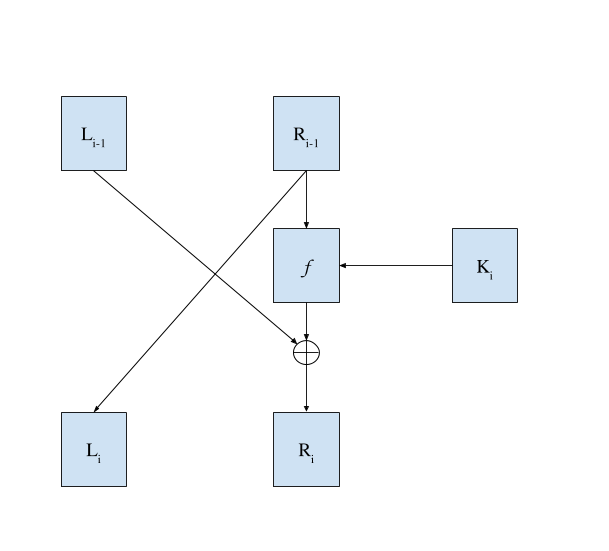
\includegraphics[width=0.75\textwidth]{./feistel}
\end{center}
\caption{Feistel system structure.}
\end{figure}

DES is a block cipher and a Feistel system. 
Named after Horst Feistel who was on the team which created LUCIFER.
Feistel systems tend to have many similiar structures to them.
These include bit permutations, Multiple XORs and Substitution boxes.
The intent of any Feistel system is to create large changes in the plaintext with ever round.
However often as a consquence of their structure, encryption and decryption schemes are nearly identical.


\section{Simplified DES (SDES) }

The simplified version of the Data encryption standard ( SDES ) that is presented here uses four rounds and two substitution boxes to encrypt plaintext.
It is a block cypher just like DES, but instead of 64-bit block it uses 12-bit blocks. 
The key is also much smaller only 9-bits ( Although only 8-bits are used every round).

\subsection{Encryption and Decryption}

\begin{figure}[ht]
\begin{center}
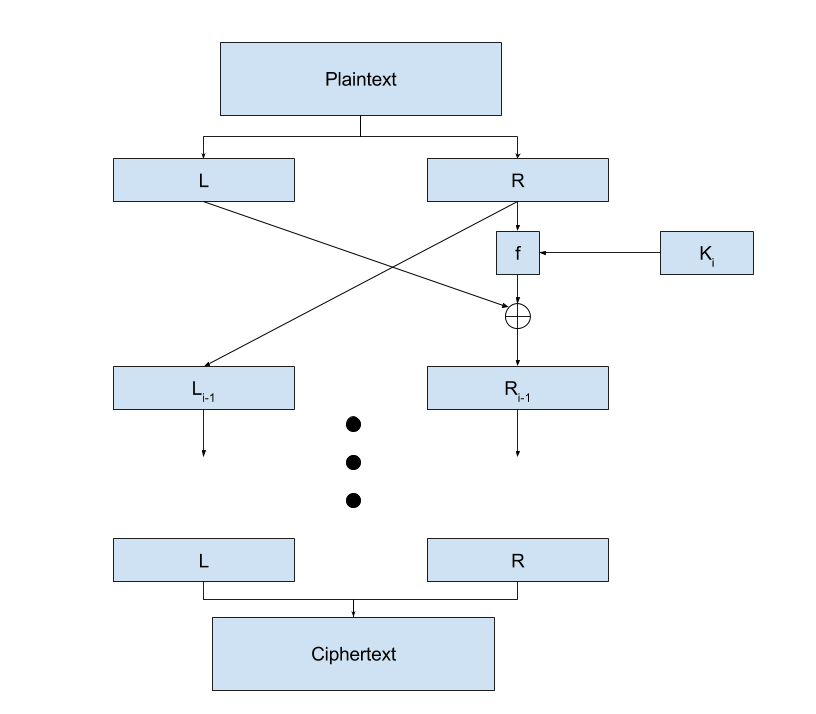
\includegraphics[width=0.75\textwidth]{./SDESflow}
\end{center}
\caption{Feistel system structure.}
\end{figure}

\begin{figure}[ht]
\begin{center}
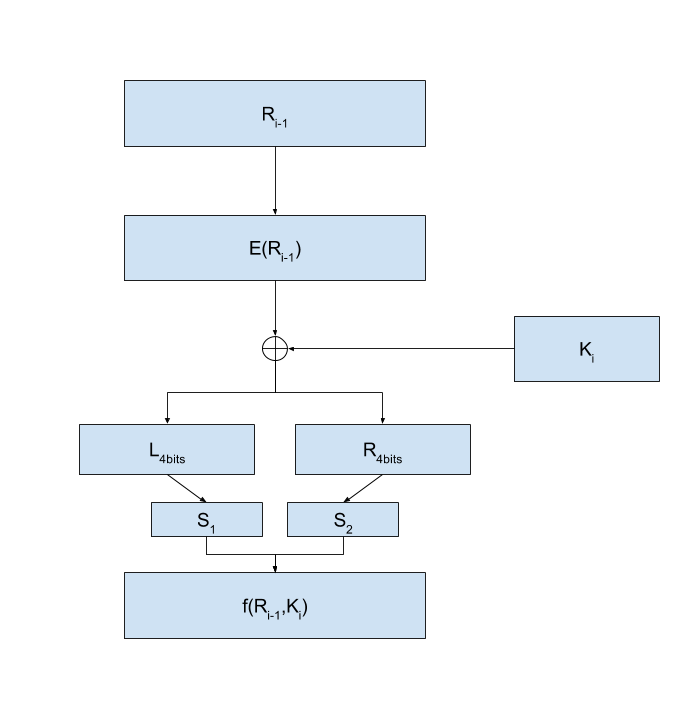
\includegraphics[width=0.5\textwidth]{./fFunc}
\end{center}
\caption{ One round of the SDES Feisel System.}
\end{figure}



\section{64-bit DES}

\begin{figure}[ht]
\begin{center}
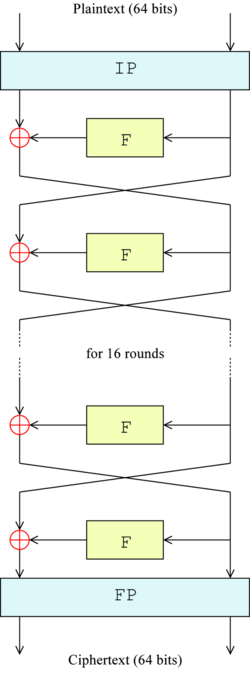
\includegraphics[width=0.5\textwidth]{./DESAlgo}
\end{center}
\caption{DES Algorithm Overview}
\end{figure}

\begin{figure}[ht]
\begin{center}
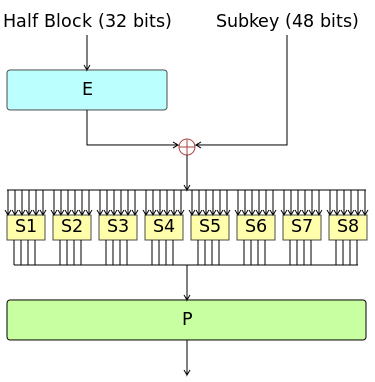
\includegraphics[width=0.4\textwidth]{./FFfunc}
\end{center}
\caption{DES Function $f(R_{i-1},K_i)$}
\end{figure}

\begin{figure}[ht]
\begin{center}
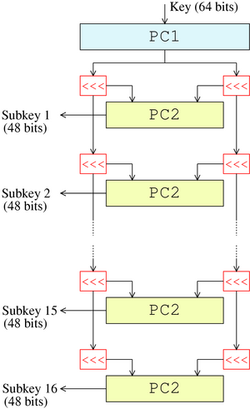
\includegraphics[width=0.3\textwidth]{./DESkey}
\end{center}
\caption{DES's key scheduler}
\end{figure}

\subsection{Encryption}
\subsection{Decryption}


% !TEX root = DesignDocument.tex

\chapter{RSA (Rivest-Shamir-Adleman)}

RSA is a public key cryptosystem which allows for asymmetric key encryption.
RSA uses large primes to create a system in which a person can publish public key
that consists of an encryption exponent and a modulus.
With these any person can send a message that only the owner of the private key will be able to decrypt. 

\subsection{Implementation}
This package contains an implementation of RSA in 3 convenient programs.
To build this packages RSA implementation navigate to \textit{Cryptosuite/RSA/} and fun \textbf{make}, this will create \textit{keygen}, \textit{ encrypt}, and \textit{decrypt}.

\begin{verbatim}
$ ./keygen 2048 > keyfile
$ ./keygen 2041 > keyfile
   Keysize must be divisible by 8 and greater than 512
$ ./encrypt keyfile < plaintext > ciphertext
$ ./decrypt keyfile < ciphertext
\end{verbatim}

\section{ Key Generation}

This implementation of  RSA allows for variable key size so long as size of the key is greater than 512. This restriction is due to how $e$ is created. Which will be discussed later.

The keys for this implementation of RSA is quite standard when viewing from a high level.
First two primes $p$ and $q$ are chosen based on user specifications on keysize. Then an $e$ is chosen with $gcd(e,(p-1)(q-1)) = 1$. 
Then the program finds the modular inverse of $e$ such that $de \equiv \pmod{(p-1)(q-1)} $.
The program then creates a keyfile in the format,
\begin{verbatim}
KEYSIZE
PUBLICKEY
ENCRYPTION_MODULUS
PRIVATEKEY
\end{verbatim}
and writes it to standard out.

\subsection{Implementation}
For the most part this is standard deterministic simple math, except for choosing $e$.
For this implementation I chose to use a standard value of $65537 = 2^{16} +1$.
This saves the time of having to look around for an $e$ that is relatively prime with $(p-1)(q-1)$.
During my research for this project i found that an $e$ with short bit-length and a small Hamming weight results in a more efficient encryption and that 65537 was a common choice. 
Additionally this $e$ is prime, meaning that there is less of a chance that $(p-1)(q-1)|e$

It is important to note that both the public key and private key are output on the same stream. 
Separation of these values is not considered.
The values for the public key, encryption modulus and private key are printed as base-16 hexadecimal strings.

\section{ Encryption }

Encryption is performed as it is stated in the algorithm, taking at most keysize bits of message interpreted as an integer and raised to the power of the public key mod the encryption modulus.

\subsection{Implementation}

The program for encrypting text begins by making sure the user has provided the program with a key file and that it holds valid data.
This data validation only goes as far as making sure that the keysize is at least a number, and then that the public key and modulus are at least interpretable as base-16 hexadecimal numbers. 
Other than these factors the keyfile is assumed to be correct.

After parsing the key file, the program begins to read from \textbf{stdin}. 
This read is buffered and attempts to read a number of bytes equal to the keysize divided by eight.
This is why the keysize needs to be divisible by eight, so sub-char parsing need not be done.
The received buffer is then directly placed into a GMP integer and raised to the power of the Public key.
The resultant integer is written to \textbf{stdout} as a hexadecimal string followed by a new line.
The new line is important during decryption as the implementation will detail.

This process continues until an \textbf{EOF} is reached at which point the program exits.


\section{ Decryption }

Decryption is also performed in a rather standard form. Taking in ciphertext of keysize bits interpreted as an integer raised to the decryption exponent which yields the message.

\subsection{Implementation}

The program for encrypting text begins by making sure the user has provided the program with a key file and that it holds valid data.
This data validation only goes as far as making sure that the keysize is at least a number, and then that the private key is at least interpretable as base-16 hexadecimal numbers. 
Other than these factors the keyfile is assumed to be correct.


After parsing the key file, the program begins to read from \textbf{stdin}. 

The program reads line by line for input that can be interpreted as a hexadecimal string.
That string is imported into a GMP integer and raised to the power of the decryption exponent which yields the plaintext as an integer.
The resultant integer is exported to a buffer using \textbf{mpz\_export()} and written to \textbf{stdout}.

This process continues until an \textbf{EOF} is reached at which point the program exits.


\appendix

\backmatter

\end{document}
